À la fin de la cinquième semaine, une planification initiale a été rendue.
Tout au long du projet, les tâches réalisées chaque jour ont été consignées. Cette démarche permet, à la fin, de comparer les tâches prévues et le temps estimé par rapport à ce qui s'est réellement passé.
Cette comparaison s'avère très intéressante, car elle permet de déterminer si les estimations étaient plutôt optimistes ou pessimistes.

Il est essentiel de noter que certains points ont été ajoutés après la cinquième semaine dans le cahier des charges, sous forme de liste sur la plateforme Gaps.
C'est pourquoi plusieurs tâches n'étaient pas prévues initialement.

Dans les planifications qui suivent, il convient de noter que la planification n'est pas parfaitement exacte.
En effet, la durée des journées pendant le semestre est de 8.125 heures.
Cependant, pour faciliter le comptage du nombre d'heures, un arrondi à 8 heures a été effectué dans le comptage du nombre d'heures.

\newpage
\subsection{Planification initiale}

\begin{figure}[H]
    \centering
    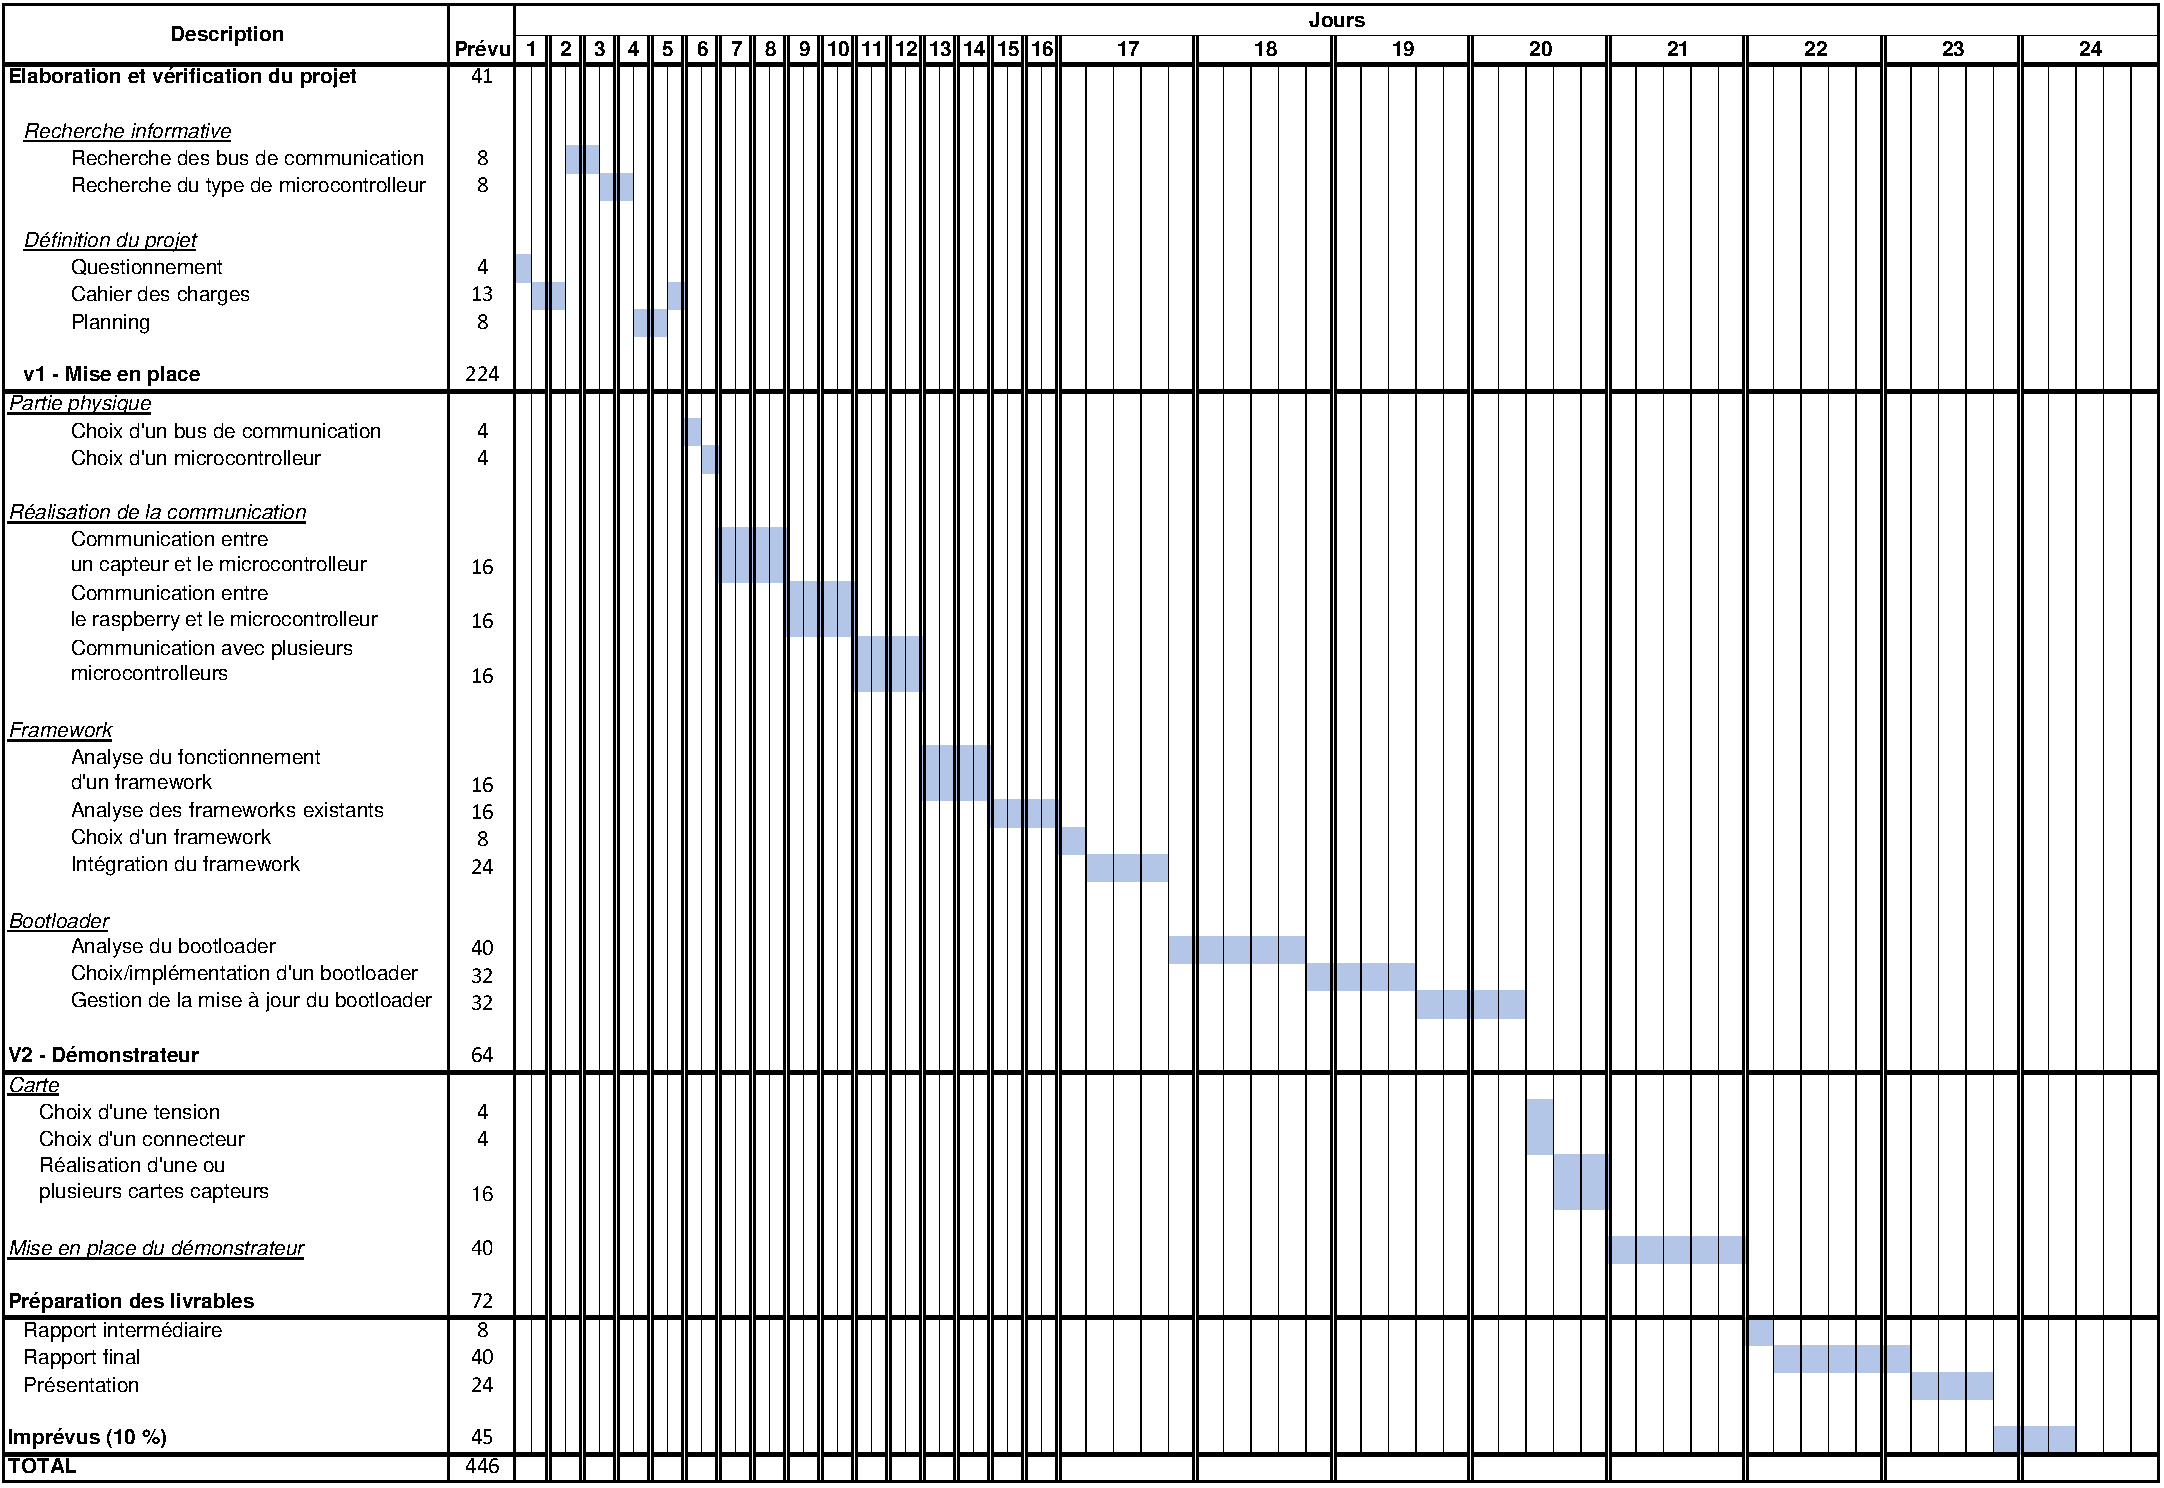
\includegraphics[angle=90,origin=c,scale=0.55]{./assets/files/planning_initial.pdf}
    \caption{Planification initiale}
\end{figure}

\newpage
\subsection{Réel}

Voici la superposition de la planification initiale avec ce qui a été réellement accompli. La couleur bleu clair représente ce qui est prévu, tandis que la couleur bleu foncé représente ce qui s'est réellement passé.

\begin{figure}[H]
    \centering
    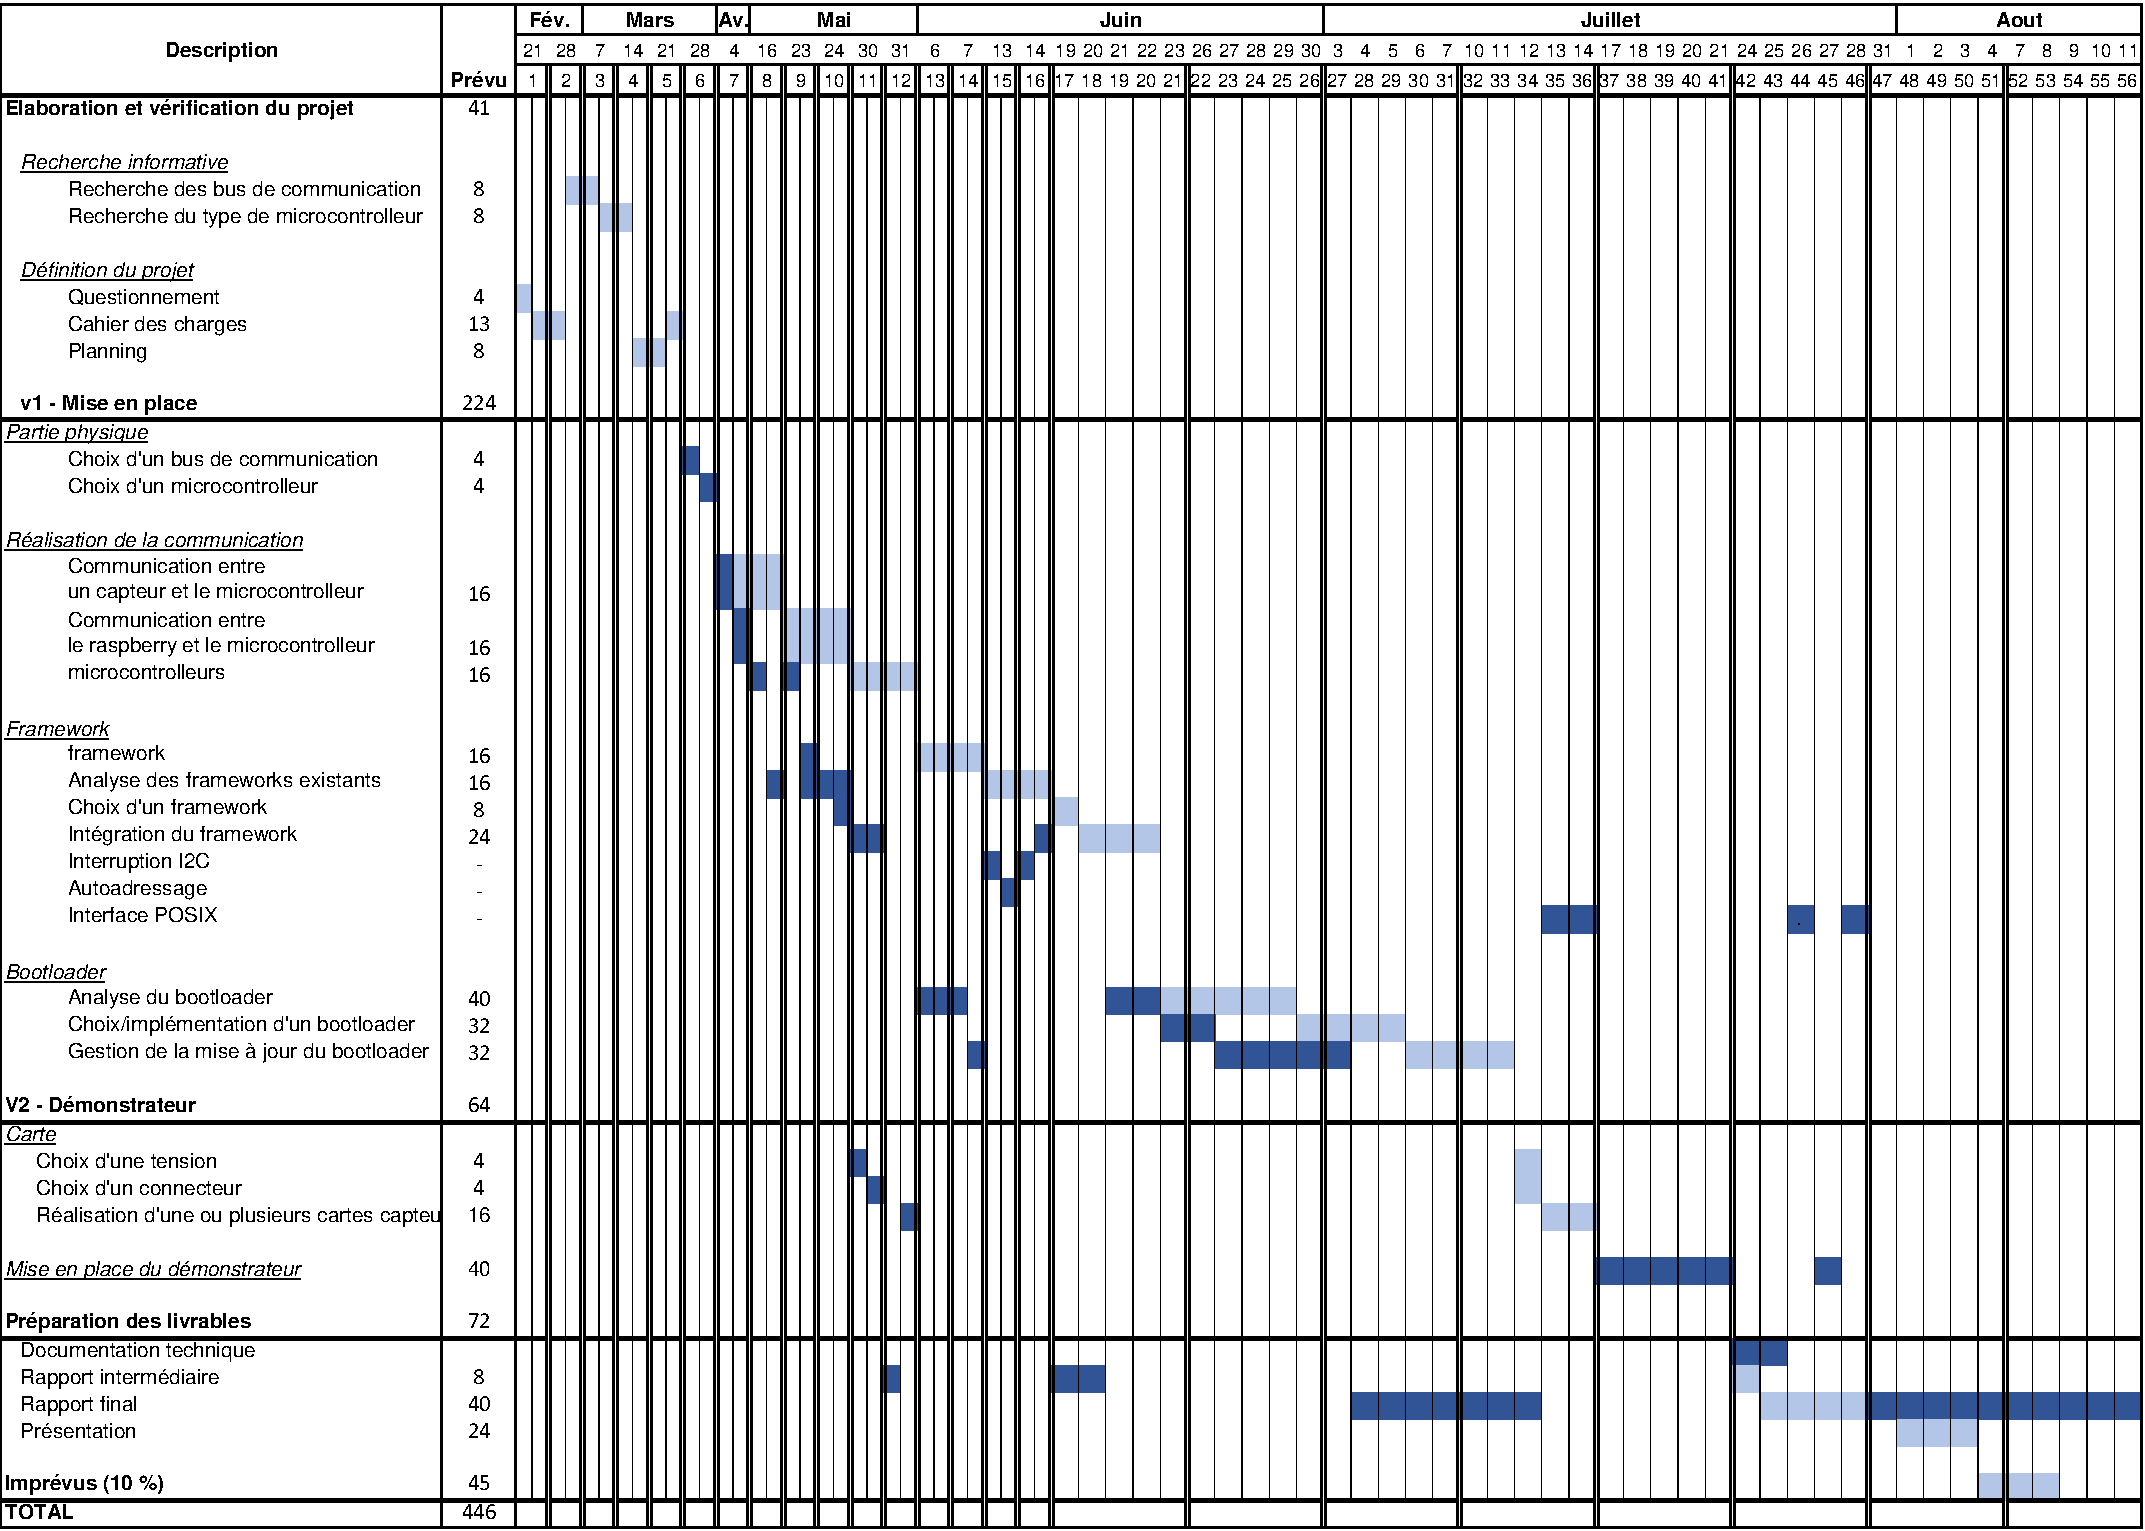
\includegraphics[angle=90,origin=c,scale=0.54]{./assets/files/planning_reel.pdf}
    \caption{Confrontation des faits}
\end{figure}

\newpage
\subsection{Comparaison}

Les cinq premières semaines n'ont pas été définies de manière précise, car la mise en place et la planification se sont faites à ce moment-là.

Concernant la partie \textit{Partie physique}, le temps réel prévu correspond au temps réel effectivement utilisé, ce qui est satisfaisant.

Pour la partie \textit{Réalisation de la communication}, le temps réel a été beaucoup plus court que prévu.
Cela s'explique par la facilité de mise en \oe{}uvre et la disponibilité de tutoriels sur internet pour les cartes Nucleo STM32.

Concernant la partie \textit{\gls{framework}}, le temps réel a également été plus court que prévu.
Cependant, des tâches annexes non prévues lors des cinq premières semaines ont été ajoutées.
Malgré cela, le temps total pour cette partie, y compris les nouvelles tâches, a été de 64 heures au lieu des 58 heures prévues initialement.

La partie \textit{Bootloader} a réellement pris 88 heures alors que 104 heures étaient prévues.
Cela s'explique par le fait que pendant les séances, il a été mentionné que cette partie serait importante dans le travail de bachelor, ce qui a justifié l'estimation initiale.

Concernant la partie \textit{Carte}, le début des travaux a été anticipé par rapport à la planification initiale.
Cette précaution était nécessaire car certains employés de la \gls{heig} étaient en vacances pendant l'été, ce qui aurait pu entraîner des blocages.
L'estimation du temps s'est avérée assez précise dans ce cas.

La partie \textit{Mise en place du démonstrateur} prévue à 40 heures a finalement pris 8 heures de plus.
Cela est dû à l'apprentissage des outils à utiliser, la nécessité de tester plusieurs éléments en même temps (carte, débogueur ST-LINK, câble Tag-Connect et adaptateur ST-Link à Tag-Connect) et la réalisation de câbles et d'un adaptateur pour connecter le circuit imprimé à la place des câbles Dupont.

Enfin, la partie \textit{Préparation des livrables} a été ajustée en cours de projet.
La documentation technique n'était pas initialement prévue, mais elle a été ajoutée.
De plus, le temps alloué au rapport a été bien plus important que prévu.
Les 50 heures de travail conseillées n'ont pas été suffisantes pour atteindre le résultat attendu.
La présentation initialement prévue n'était pas incluse dans les 450 heures du projet, et elle doit être réalisée entre la fin du travail de bachelor et la présentation finale.

En conclusion, il est observé que la réalisation de la plupart des aspects techniques a été plus rapide que prévu, tandis que la documentation a demandé davantage de temps.
De plus, des éléments techniques non initialement envisagés ont été intégrés au projet, entraînant un investissement en temps supplémentaire.

\subsection{Conclusion}

Au final, tous les objectifs du cahier des charges ont été réalisés.
De plus, un objectif dans la catégorie \textit{Si le temps le permet} a été accompli, celui-ci étant de \textit{Réaliser une carte électronique dédiée avec un capteur}.
Néanmoins, l'accomplissement de cet objectif a nécessité un temps considérable de 60 heures, ce qui représente environ 13\% du temps total du projet de 450 heures.
Le deuxième objectif de la catégorie \textit{Si le temps le permet} concerne le \textit{CI/CD}, qui a été expliqué dans le projet mais n'a pas été mis en place.
Il a été jugé plus approprié de consacrer davantage de temps au rapport plutôt que de s'efforcer à tout prix de réaliser tous les objectifs supplémentaires.